\documentclass[conference]{../cls/IEEEtran}

\usepackage{graphics}

\begin{document}

\title{Behavior Estimation Framework for Distributed Decision Making on Cooperative Vehicle Routing}

\author{
	\IEEEauthorblockN{Dominik Ascher}
	\IEEEauthorblockA{
		Chair IV: Software \& Systems Engineering\\
		Technische Universit\"at M\"unchen\\
		Boltzmannstr.\ 3, 85748 Garching, Germany\\
		Email: ds.ascher@gmail.com
	}
	\and
	\IEEEauthorblockN{Georg Hackenberg}
	\IEEEauthorblockA{
		Chair IV: Software \& Systems Engineering\\
		Technische Universit\"at M\"unchen\\
		Boltzmannstr.\ 3, 85748 Garching, Germany\\
		Email: hackenbe@in.tum.de
	}
}

\maketitle

\begin{abstract}
Many visions and ideas arise from increasing computational and communicational capabilities of recent and future automotive vehicles.
Early studies have to show the feasability and potential of these ideas to foster future research and development.
\end{abstract}

\begin{IEEEkeywords}
Rapid prototyping.
\end{IEEEkeywords}

\section{Motivation}

State of the art

Problem

Contribution

In the following we describe shortly the underlying framework before explaining the cooperative vehicle routing demonstrator.

\section{Behavior Estimation Framework}

\begin{figure}[b]
	\centering
	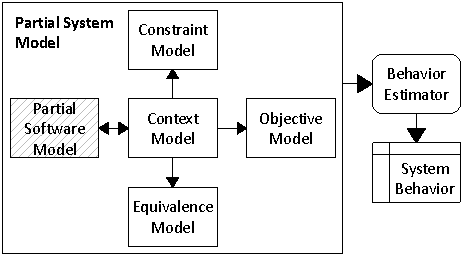
\includegraphics{../gfx/framework.pdf}
	\caption{Overview of the estimation framework including partial system model, behavior estimator and system behavior.}
\end{figure}

Annotation approach \cite{Hackenberg2012}

Estimation algorithm

\section{Cooperative Vehicle Routing}

Model architecture: Context (i.e.\ vehicle) component, constraint component, objective component, control component, equivalence component.

Component behavior: Speed selection, edge selection, edge-based collision detection, energy consumption, etc.

Behavior estimation: One basic case (single vehicle, two routes) and one more complex case (multiple vehicles).

\section{Conclusion and Outlook}

Great stuff! :)

\bibliographystyle{../bst/IEEEtran}
\bibliography{ICCVE-2014}

\end{document}
